% !TEX root = mythesis.tex

%==============================================================================
\chapter{Methods}
\label{sec:methods}
%==============================================================================
% History
% Pros & Cons
% Ergodisity (Avoiding problems)
% Application of HMC onto the lattice
% Bootstrap
\section{Hybrid Monte Carlo}
% MCMC
%% Why these algos are better that a MC
%% Markov chain definition
%%% Stationary distribution
%%% Detailed balance
% Hamiltonian Dynamics
%% Leapfrog integrator
% Metropolis Hastings
% Summary of the algo
The Hybrid (Hamiltonian) Monte Carlo (HMC) algorithm is the workhorse of modern Lattice QCD simulations and other Hamiltonian theories~\cite{hmccm}. This is due to the difficulty of simulating fermions with their anti-commuting nature using standard Monte Carlo (MC) methods. The major advantage of HMC over other methods is that this algorithm updates the system globally instead of the local updates that standard MC methods use. Moreover, the method is exact, meaning it does not have and truncation errors and the ensemble averages do not depend on the integration step size. These two advantages reduce the critical slowing down from which the other MC methods suffer. In the following subsections we will discuss in some detail the individual methods and algorithms that are involved in the creation of HMC.

\subsection{Markov Chain Monte Carlo}

Monte Carlo algorithms in general are used in quantum field theory to calculate the expectation value of an observable, leveraging the law of large numbers

\begin{equation}
    \langle\mathcal{O}\rangle = \frac{1}{Z} \int d\phi \mathcal{O} e^{-S[\phi]},
\end{equation}
where
\begin{equation}
    Z = \int d\phi e^{-S[\phi]}
\end{equation}
This is done by sampling $\phi$ fields from a distribution
\begin{equation}
    P(\phi) = \frac{1}{Z} \int d\phi e^{-S[\phi]}
\end{equation}
and then calculating the average
\begin{equation}
    \overline{\mathcal{O}} \equiv \frac{1}{N}\sum^{N}_{n=1} \mathcal{O}(\phi_n)
    \label{eq:ensamble_average}
\end{equation}
And in the limit of $N \to \infty$, we get the relation
\begin{equation}
    \overline{\mathcal{O}} = \langle\mathcal{O}\rangle + \mathrm{O}(1/\sqrt{N})
\end{equation}

Making simulations by sampling directly from distributions could prove very costly and practically impossible. This is because the phase space of the target distribution might be too big to explore it all (curse of dimensionality). A much better way to explore the phase space is by progressively uncovering the regions of interest~\cite{mhexpl}, which could be done by the use of Markov Chain.

The Markov Chain~\cite{intromarkov} is defined as a sequence of random variables $X_n$, where every next element is generated from the previous element in the chain by a transition matrix $P_{ii+1}$
\begin{equation}
    X_0 \xrightarrow{P_{01}} X_1 \xrightarrow{P_{12}} X_2 \xrightarrow{P_{23}} \cdots \xrightarrow{P_{n-1n}} X_n
\end{equation}
If the chain is ergodic and positive recurrent, then the detailed balance condition ensures that the Markov chain converges to a unique stationary distribution $p$
\begin{equation}
    p(X_i) P_{ij} = p(X_j) P_{ji}
\end{equation}

All Monte Carlo algorithm that use this method of random variable sampling are called Markov Chain Monte Carlo (MCMC) algorithms. HMC is a MCMC algorithm since we use a Markov chain to explore the target distribution, from which we draw the $\phi$ fields.

\subsection{Hamilton Dynamics}

The proposed updates to the system that we work with, must not change the energy. This is exactly what the Hamilton dynamics do. They preserve the Hamiltonian (the energy of the system). Therefore, we define Hamiltonian dynamics to evolve our $\phi(\tau)$, where $\tau$ is an evolution parameter~\cite{hmc}. We introduce conjugate momenta $\pi(\tau)$ and a Hamiltonian 
\begin{equation}
    H(\phi,\pi) \equiv \frac{1}{2}\pi^2 + S(\phi),
\end{equation}
where $S(\phi)$ is the action. Now, can use the equations of motion to evolve $\phi$
\begin{equation}
    \dot{\phi} = \frac{\delta H}{\delta \pi} \qquad \dot{\pi} = - \frac{\delta H}{\delta \phi} = - \frac{\delta S}{\delta \phi}
    \label{eq:eom}
\end{equation}
The initial momentum $\pi$ is selected from a Gaussian distribution function with mean zero and unit variance. Then the whole system is evolved though the ($\phi,\pi$)-phase space. There are a lot of algorithms that can be used to solve (\ref{eq:eom}) but the most common method is the Leapfrog integrator. It is reversible and preserves the area which makes it a perfect candidate, due to the detailed balance requirement. The algorithm is simple; with initial half-step
\begin{equation}
    \pi\left(\frac{\delta\tau}{2}\right) = \pi\left(0\right) - \left[ \frac{\delta S(0)}{\delta\phi} \right] \frac{\delta\tau}{2}
\end{equation}
This is followed by $n=\frac{\tau_0}{\delta\tau}$ steps in $\phi$ and $n-1$ in $\pi$
\begin{equation}
    \begin{aligned}
        \phi(\tau+\delta\tau) = \phi(\tau) + \pi(\tau+\frac{\delta\tau}{2})\delta\tau
        \\
        \pi(\tau+\frac{\delta\tau}{2}) = \pi(\tau-\frac{\delta\tau}{2}) - \left[ \frac{\delta S(\tau)}{\delta\phi} \right] \delta\tau
    \end{aligned}
\end{equation}
and again half-step in $\pi$
\begin{equation}
    \pi(\tau_0) = \pi(\tau_0-\frac{\delta\tau}{2}) - \left[ \frac{\delta S(\tau_0)}{\delta\phi} \right] \frac{\delta\tau}{2}
\end{equation}
On Figure \ref{fig:leapfrog} is show a schematic view of the leapfrog integration process.
\begin{figure}[htbp]
    \centerline{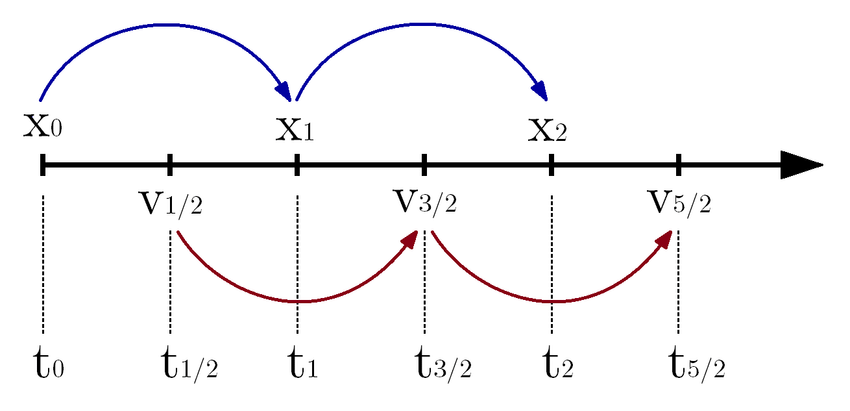
\includegraphics[width=0.5\linewidth]{leapfrog.png}}
    \caption{Leapfrog integration process. The scheme represents one integration trajectory. On each step of evolution, one of the variables lead the other by a half step, and they update each other. %https://www.researchgate.net/figure/Schematics-describing-how-the-leapfrog-algorithm-works-Position-and-velocity-leap-each_fig1_346972792}
    }
    \label{fig:leapfrog}
\end{figure}

\subsection{Metropolis-Hastings}

A Metropolis-Hastings accept/reject algorithm~\cite{mhog, mhexpl} is used to construct a Markov chain with a stationary distribution $p(X)$. This is done by having a candidate element with transition probability $P_{acc}$. The accepted proposal is the new element of the chain, but if it is rejected the old element becomes the new one. This algorithm preserves the stationary distribution if the chain is irreducible.

\begin{figure}[htbp]
    \centerline{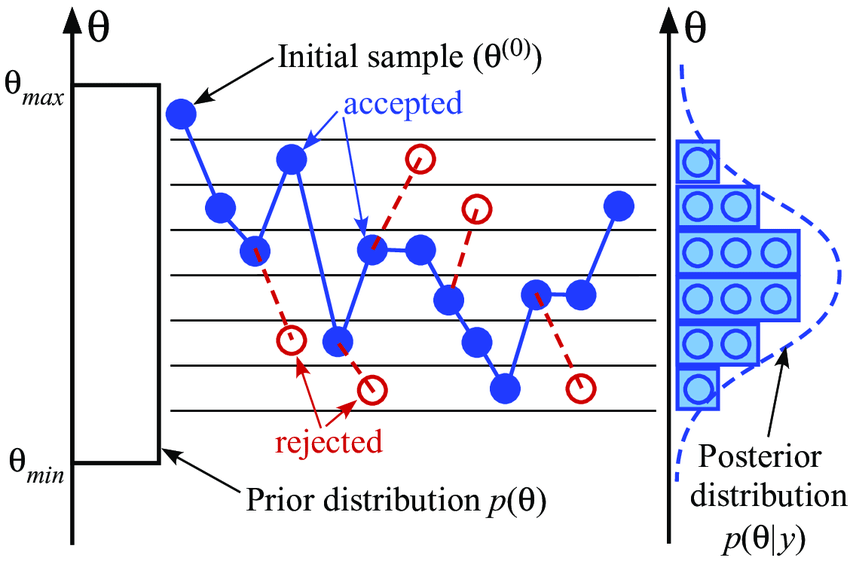
\includegraphics[width=0.5\linewidth]{
        Metropolis-Hastings-MCMC.png}}
    \caption{Metropolis-Hastings process for generating a Markov chain with a target distribution. The scheme represents the transition from an initial probability distribution to a target one. On each step, the accept/reject step is performed on the candidate element. The first element of the Markov chain is drawn from the starting distribution. The whole process is repeated until all sampled elements are representative of the new distribution. %https://www.researchgate.net/figure/Illustration-of-the-Markov-chain-Monte-Carlo-with-Metropolis-Hastings-MCMC-MH-procedure_fig6_338363810
    }
    \label{fig:mn-mcmc}
\end{figure}
This algorithm is used in HMC as an accept/reject step on the new proposed $\phi$ field. The candidate is accepted with probability 
\begin{equation}
    P_{acc} = min(1, \exp(\delta H)),
\end{equation}
where $\delta H = H' - H$ is the difference of the final and the starting Hamiltonians. This difference $\delta H$ is not zero because of the finite number of integration steps. The whole process repeats until we are satisfied by the number of configuration in the constructed Markov chain which will be averaged in (\ref{eq:ensamble_average}). On Figure \ref{fig:mn-mcmc} is shown how the Markov chain is constructed using the Metropolis-Hastings accept/reject algorithm. This acceptance rate can be tuned by the number of integration steps which can make the exploration of the phase space easier.

\subsection{Summary of the Algorithm}

We have discussed until now how we compute numerically the expectation value (\ref{eq:ensamble_average}) of an observable using MC algorithms. We also saw a better approach to draw from distributions that are difficult to sample using MCMC methods. This approach uses proposed elements which construct a Markov chain. These candidates can be found by leveraging the Hamilton dynamics and can be accepted with a probability $P_{acc}$. All of these methods culminate in the HMC algorithm~\cite{hmc}, which is summarized in Algorithm (\ref{alg:hmc})

\begin{algorithm}
    \caption{Hybrid Monte Carlo}
    \begin{algorithmic}[1]
        \State Initialize  $\tau, N_{max}$
        \State Initialize $\phi_0, \pi_0$
        \State Sample $\pi_0 \sim \mathcal{N}(0,1)$

        \State Set $(\phi_{i}, \pi_{i}) = (\phi_0, \pi'_0)$ \Comment{Initial Condition}
        \While{$i < N_{max}$}  \Comment{Markov Chain}
            \State Calculate $H(\phi_{i}, \pi_{i})$
            \State Leapfrog $(\phi', \pi') \xleftarrow{\tau_\text{steps}} (\phi_{i}, \pi_{i})$ \Comment{Find a candidate}
            \State Calculate $H'(\phi',\pi')$
            \State Calculate $\delta H = H'(\phi',\pi')-H(\phi_{i},\pi_{i})$
            \If{$P_{acc} = min(1, \exp(-\delta H))$} \Comment{Accept/Reject step}
                \State Set $(\phi_{i+1}, \pi_{i+1}) = (\phi', \pi')$
                \Else
                \State Set $(\phi_{i+1}, \pi_{i+1}) = (\phi_{i}, \pi_{i})$
            \EndIf
        \State Set $i = i + 1$
        \EndWhile
    \end{algorithmic}
    \label{alg:hmc}
    \end{algorithm}

\section{Linear Solvers}

We saw in Section \ref{sec:corr_func} that if we want to numerically compute the expectation value of the correlation functions, we must work with a lot of inverse matrices. Therefore, we must find a method for inverting matrices, which could be either a direct or an iterative method of solving linear systems of equations
\begin{equation}
    Ax = b
    \label{eq:lineq}
\end{equation}
In this work, we use the latter methods, namely the Flexible Generalized Minimum Residual (FGMRES) method~\cite{fgmresart}. This method can be used for any invertible matrix, but it usually converges very slow. Some even make an analogy with a tank, because it is slow but robust and if there is a solution, it will find it. A solution to the speed of the algorithm is to use a preconditioner. We have chosen to use the Conjugate Gradient (CG) method~\cite{cgbook}. In the next subsections, we will discuss how both methods work. This includes the application of CG as a preconditioner to FGMRES.

\subsection{Conjugate Gradient}

Conjugate gradient is used as an iterative method of solving linear systems of equations that are too large to solve directly. And more precisely with real,  positive-definite usually with sparse matrices. The idea of the algorithm is to have a number of orthogonal search directions. And each search direction is explored fully before going to the next. This method can be viewed as an improved version of the gradient descent method, where the search is always done in the direction of the gradient. A comparison between the methods is shown on Figure \ref{fig:cg_comp}.
\begin{figure}[htbp]
    \centerline{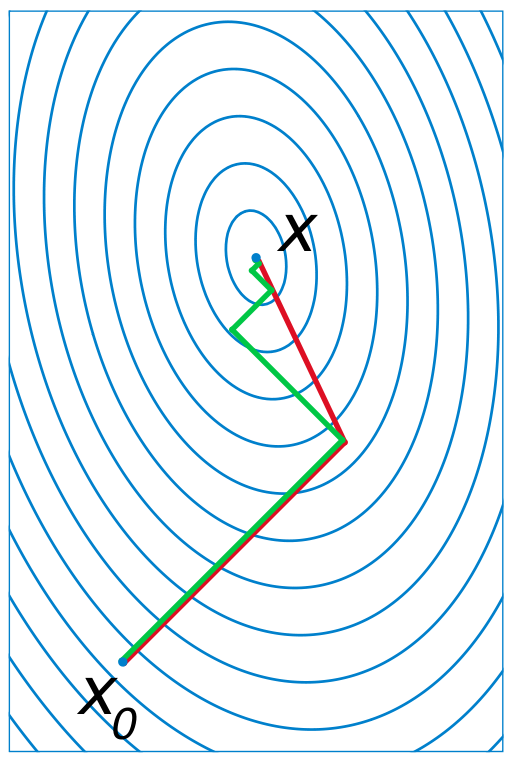
\includegraphics[width=0.5\linewidth]{CG_comparison.png}}
    \caption{Comparison between Conjugate gradient (red) and Gradient descent (green) methods. This is done with the same starting point and an optimal step size for the GD.}
    \label{fig:cg_comp}
\end{figure}

The way we start with the derivation is with the definition of an $A$-matrix inner product for any two vectors
\begin{equation}
    \left( u, v \right)_A = u^\top A v
    \label{eq:cg_constraint}
\end{equation}
and if the product is equal to zero, these vectors are conjugate. Now, we can make a basis of mutually conjugate vectors $\{ p_i \}$, so that we could represent the solution $x'$ of (\ref{eq:lineq}) as a linear combination
\begin{equation}
    x' = \sum_i \alpha_i p_i,
\end{equation}
where
\begin{equation}
    \alpha_i = \frac{\left( p_i, b \right)}{\left( p_i, p_i \right)_A}
\end{equation}

In most cases it is not possible to get the exact result, due to round off error, and one must be content with an approximation of the true result. This means that we do not actually need all conjugate vectors of the basis in order to find a good solution, but we can progressively add more vectors until we are satisfied with the solution.

To show this, we start again with (\ref{eq:lineq}) which is the minimizer (gradient) of a quadratic function
\begin{equation}
    \begin{aligned}
        f(x) &= \frac{1}{2} x^\top A x - x^\top b
        \\
        \nabla f(x) &=  Ax - b
    \end{aligned}
\end{equation}
The goal is to find the minimum, so we define a residual 
\begin{equation}
    r_k = b - Ax_k,
\end{equation}
which measures how close we are to the minimum. And iteratively, the new residual can be computed from the previous
\begin{equation}
    r_{k+1} = r_k - \alpha_k Ap_k,
\end{equation}
where
\begin{equation}
    \alpha_k = \frac{\left( r_k, r_k \right)}{\left( p_k, p_k \right)_A}
\end{equation}
In the Steepest descent method, we use the residuals as search directions, but the improved version that we work with, puts a constraint (\ref{eq:cg_constraint}) on the searches. In order to ensure that the directions are linearly independent, we perform some form of Gram-Schmidt orthogonalization procedure on the residuals where every new $A$-orthogonal vector can be calculated from the previous
\begin{equation}
    p_{k+1} = r_{k+1} + \beta p_k,
\end{equation}
where
\begin{align}
    \beta &= \frac{\left( r_{k+1}, r_{k+1} \right)}{\left( r_k, r_k \right)}
\end{align}
And the new solution can be found by
\begin{equation}
    x_{k+1} = x_k + \alpha_k p_k
\end{equation}
A detailed derivation of CG can be found in~\cite{cgbook}. The whole method can be implemented in an algorithm which can be written in pseudocode (Algorithm \ref{alg:cg}) like

\begin{algorithm}
    \caption{Conjugate Gradient}
    \begin{algorithmic}[1]
        \State Initialize  $A, x_0, b$
        \State Initialize $\epsilon$ \Comment{Convergence criteria}
        \State Set $r_0 = b - Ax_0$ \Comment{Initial Condition}
        \State Set $p_0 = r_0$ \Comment{Initial Search Direction}
        \While{$r_{k+1} > \epsilon$}
            \State Set $\alpha_k = \frac{\left( r_k, r_k \right)}{\left( Ap_k, p_k \right)}$
            \State Update $x_{k+1} = x_k + \alpha_k p_k$
            \State Update $r_{k+1} = r_k - \alpha_k Ap_k$
            \State Set $\beta = \frac{\left( r_{k+1}, r_{k+1} \right)}{\left( r_k, r_k \right)}$
            \State Update $p_{k+1} = r_{k+1} + \beta p_k$
        \EndWhile
    \end{algorithmic}
    \label{alg:cg}
    \end{algorithm}

\subsection{Flexible Generalized Minimum Residual}

This method is a variant of the GMRES method with preconditioning. It is called flexible because it can have different preconditioning on each step of the algorithm, whereas in the previous versions it can have only the same preconditioner on each step. It will be easier to understand the whole FGMRES method if we first explain how the preconditioned GMRES works.

The GMRES algorithm is trying to find an approximate solution to (\ref{eq:lineq}) by building a Krylov subspace, which is defined as
\begin{equation}
    \mathcal{K}_n = \mathcal{K}_n (A, r_0) = span \{ r_0, Ar_0, A^2r_0,\hdots, A^{n-1}r_0 \}
\end{equation}
An important property of this subspace is that the vectors are linearly independent, therefore we can use them as a basis to represent our solution. This is done by applying an Arnoldi method, which can find an orthonormal basis in $\mathcal{K}_n$. The process creates a matrix $\bar{H}_m = H_{(m+1)\times m}$. This matrix is used for minimizing the residual $y_m = min(\beta e_1 - \bar{H}_m y)$, which updates the approximation of the solution $x_m = x_0 + Z_my_m$.

As it was written before, this method is robust but slow. So, in order to improve the speed of convergence, we can precondition the original matrix. In FGMRES, we use the right preconditioning
\begin{equation}
    AM^{-1}(Mx) = b,
\end{equation}
where $M$ is a matrix that can be found very easy with another algorithm by solving $Mz = v$. One could use a lot of different methods for preconditioning. They could be not only one-step methods but also iterative techniques like SSOR, ADI, CG, and even GMRES. The detailed derivation of the method can be found in~\cite{fgmresart}, but here we can only show the general idea of the algorithm with a pseudocode (Algorithm \ref{alg:fgmres})

\begin{algorithm}
    \caption{Flexible Generalized Minimum Residual}
    \begin{algorithmic}[1]
        \State Initialize $\epsilon$ \Comment{Convergence criteria}
        \State Initialize  $A, x_0, b$
        \State Initialize $\bar{H}_m$
        \While{$r_m > \epsilon$}
            \State Compute $r_0 = b - Ax_0$
            \State Set $\beta = ||r_0||$
            \State Compute $v_1 = \frac{r_0}{\beta}$
            \For{$j = 1, 2, ..., m$} \Comment{Arnoldi process}
                \State Compute $z_j = M^{-1}_jv_j$ \Comment{Preconditioning (could be different on every step)}
                \State Compute $w = Az_j$
                \For{$i = 1, ..., j$}
                    \State Compute $h_{i,j} = (w, v_i)$
                    \State Compute $w = w - h_{i,j}v_i$
                \EndFor
                \State Set $h_{j+1,j} = ||w||$
                \State Set $v_{j+1} = \frac{w}{h_{j+1,j}}$
            \EndFor
            \State Set $Z_m = [z_1, ..., z_m]$
            \State Compute $y_m = min(\beta e_1 - \bar{H}_m y)$ \Comment{Least square minimization}
            \State Update $x_m = x_0 + Z_my_m$
            \State Update $r_m = b - Ax_m$
            \State Set $x_0 = x_m$
        \EndWhile
    \end{algorithmic}
    \label{alg:fgmres}
    \end{algorithm}
